\documentclass[conference]{IEEEtran}

\usepackage{amsmath,amssymb,amsfonts}
\usepackage{graphicx}
\usepackage{booktabs}
\usepackage{siunitx}
\usepackage{hyperref}
\usepackage{cite}
\usepackage{flushend}

\hypersetup{
    colorlinks=true,
    linkcolor=blue,
    citecolor=blue,
    urlcolor=blue
}

\begin{document}

\title{Emergent Niche Bifurcation and Convergent Trait Evolution Under Planetary Environmental Constraints: A Vectorized Agent-Based Astrobiology Simulation}

\author{
    \IEEEauthorblockN{Chetan Choudhary}
    \IEEEauthorblockA{
        Department of Computer Science\\
        Savitribai Phule Pune University, Pune, India\\
        Email: \href{mailto:chetan.choudhary.dev@gmail.com}{chetan.choudhary.dev@gmail.com}\\
        GitHub: \url{https://github.com/Parasyte23/ASTROBIO-EVO-SIM}
    }
}

\maketitle

\begin{abstract}
Predicting the metabolic and structural adaptations of putative extraterrestrial life requires modeling how planetary physics constrain evolutionary trajectories. We present a deterministic, vectorized agent-based evolutionary simulator (\texttt{astrobio-evo-sim}) parameterized with NASA/ESA planetary telemetry for Earth (control baseline), Mars, and Venus. Starting from an identical, unbiased uniform population distributed across three vertical habitat zones (subsurface, surface, and airborne), we evaluate evolutionary convergence over 20,000 hourly ticks across $n = 30$ independent random seeds per planet (90 total runs). Under a strict energy-conservation regime with metabolic upkeep trade-offs and conditional spore dormancy, all three worlds achieved 100\% survival while diverging into distinct, statistically significant biospheres (Kruskal--Wallis $p < 0.0001$ across all traits). Earth sustained a multi-niche ecosystem across all three vertical layers ($22{,}390.4 \pm 44.0$ agents), whereas Mars and Venus both purged surface life completely ($p = 1.0000$ pairwise) and bifurcated in opposite vertical directions: Mars converged to 100\% subsurface chemoautotrophs ($\text{Metab} = 0.008 \pm 0.001$) with exact cold-tolerance calibration ($\text{Therm} = 0.336 \pm 0.002$) and neutral-trait genetic drift in dormancy ($\text{SD} = 0.227$), while Venus converged to 100\% airborne photosynthetic extremophiles ($\text{Metab} = 0.993 \pm 0.000$, $\text{Acid} = 0.999 \pm 0.000$) that unexpectedly evolved high radiation shielding ($\text{Rad} = 0.963 \pm 0.002$) to survive 48-hour super-rotation nights in dormant spore state. Sensitivity sweeps further revealed linear thermodynamic tracking on Mars and a sharp extinction cliff on Venus between 144-hour and 192-hour diurnal cycles, quantitatively underscoring the role of atmospheric super-rotation in Venusian cloud habitability.
\end{abstract}

\begin{IEEEkeywords}
Artificial Life, Computational Astrobiology, Agent-Based Modeling, Evolutionary Computation, Extremophiles, Niche Partitioning
\end{IEEEkeywords}

\section{Introduction}
A central challenge in astrobiology is determining how planetary boundary conditions---such as solar irradiance, diurnal period, atmospheric density, ionizing radiation, and chemical acidity---shape the viable phenotypes of living systems \cite{seager2021venus, hassler2014mars}. While laboratory extremophile studies establish biochemical limits on Earth, they cannot easily test multi-generational evolutionary trade-offs across alternative planetary regimes.

Artificial Life (ALife) and evolutionary computation provide a complementary \textit{in silico} methodology for testing evolutionary hypotheses under controlled physical constraints \cite{adami1998introduction}. However, many evolutionary simulators either omit real-world planetary telemetry or lack strict metabolic upkeep costs, allowing digital organisms to evolve maximal defenses simultaneously without energetic penalty.

In this work, we introduce a lightweight, headless, vectorized agent-based model (ABM) grounded in NASA Planetary Fact Sheet and Mars Curiosity RAD telemetry. Rather than hardcoding planet-specific organisms, we initialize Earth, Mars, and Venus with the exact same uniform trait and habitat distributions and subject them to a universal energy-conservation law. Our primary contributions are:
\begin{enumerate}
    \item A deterministic, NumPy Structure-of-Arrays (SoA) evolutionary engine capable of simulating 50,000 agents on consumer hardware with bit-for-bit reproducibility.
    \item Multi-seed statistical proof ($n = 30$ seeds/planet) of emergent vertical niche bifurcation and convergent trait specialization across Earth, Mars, and Venus.
    \item Identification of two emergent phenomena: neutral-trait genetic drift in Martian subsurface dormancy and a nocturnal radiation-shielding trade-off in Venusian cloud spores.
    \item Sensitivity analyses quantifying thermodynamic adaptation limits on Mars and a sharp diurnal extinction threshold in the Venusian cloud deck.
\end{enumerate}

\section{Methodology}

\subsection{Planetary Parameters and Vertical Stratification}
Each planet is modeled using physical constants from the NASA Planetary Fact Sheet \cite{nasa_factsheet} and Curiosity RAD surface radiation measurements \cite{hassler2014mars}. To allow natural selection to discover viable habitats, each world is partitioned into three vertical layers: \textbf{Layer 0 (Subsurface)}, \textbf{Layer 1 (Surface)}, and \textbf{Layer 2 (Airborne)}.

\begin{itemize}
    \item \textbf{Earth (Control):} Temperate surface ($15^\circ\text{C}$), 24.0-hour day, global magnetic shielding, and moderate subsurface chemical energy.
    \item \textbf{Mars:} Cold, high-radiation surface ($-65^\circ\text{C} \pm 30^\circ\text{C}$, 24.66-hour sol), thin atmosphere ($0.00636\text{ bar}$, making buoyancy prohibitively expensive), and a radiation-shielded, geothermally buffered subsurface ($-20^\circ\text{C} \pm 2^\circ\text{C}$) rich in chemical gradients.
    \item \textbf{Venus:} Crushing, sterile surface ($464^\circ\text{C}$, $92\text{ bar}$) contrasted with a temperate 50~km cloud deck ($25^\circ\text{C} \pm 10^\circ\text{C}$) characterized by high sulfuric acid ($\text{H}_2\text{SO}_4$) acidity, low buoyancy cost, and a 96.0-hour diurnal cycle reflecting real-world atmospheric super-rotation \cite{seager2021venus}.
\end{itemize}

Diurnal temperature and solar flux at tick $t$ (where $1\text{ tick} = 1\text{ hour}$) are computed via a sinusoidal phase $\phi(t) = 2\pi t / T_{\text{day}}$:
\begin{align}
    T_l(t) &= \bar{T}_l + A_l \sin(\phi(t)), \\
    S_l(t) &= S_{l,\text{base}} \cdot \max(0, \sin(\phi(t))),
\end{align}
where $l \in \{0, 1, 2\}$ indexes the habitat layer, $\bar{T}_l$ is mean temperature, $A_l$ is diurnal amplitude, and $S_{l,\text{base}}$ is normalized solar flux.

\subsection{Organism Genome and Vectorized SoA Architecture}
To execute 90 multi-seed runs efficiently without object-oriented overhead, the population is stored in pre-allocated 1D NumPy arrays (Structure of Arrays) with fixed capacity $N_{\max} = 50{,}000$ and a boolean mask \texttt{alive}. Each organism carries five continuous, heritable genome traits normalized to $[0, 1]$---photosynthesis mode ($m$, where $0$ is pure chemosynthesis and $1$ is pure photosynthesis), radiation shielding ($r$), acid resistance ($a$), thermal tolerance ($\tau$), and dormancy threshold ($\theta$)---plus a discrete habitat layer $l \in \{0, 1, 2\}$.

\subsection{Energy Conservation and Conditional Dormancy}
To enforce a ``no free lunch'' evolutionary landscape, every defense trait incurs continuous metabolic upkeep. At each tick, local density-dependent competition in layer $l$ scales available harvest by $\rho_l = \max(0, 1 - N_l / K)$, where $K = 15{,}000$ is the per-layer carrying capacity. Potential energy harvest is:
\begin{equation}
    E_{\text{pot}} = \rho_l \left[ m S_l(t) H_{\text{solar}} + (1 - m) C_l H_{\text{chem}} \right],
\end{equation}
where $H_{\text{solar}} = 9.0$ and $H_{\text{chem}} = 3.4$. Environmental damage sums unshielded radiation, acidity, thermal deviation beyond the organism's tolerance band, and barometric pressure hazard:
\begin{align}
    E_{\text{dmg}} &= w_r R_l (1 - r) + w_a Q_l (1 - a) + w_p P_l \nonumber \\
                   &\quad + w_T \max\left(0, |T_l(t) - T_{\text{opt}}| - (B_0 + \tau B_{\max})\right),
\end{align}
with $T_{\text{opt}} = 20^\circ\text{C}$, base band $B_0 = 15^\circ\text{C}$, and max extra band $B_{\max} = 90^\circ\text{C}$.

Organisms enter a dormant spore state ($d = 1$) if and only if their energy falls below their evolved threshold \textit{and} active maintenance exceeds potential harvest:
\begin{equation}
    d = \mathbb{I}\left(E < \theta E_{\text{repro}} \;\land\; E_{\text{pot}} < E_{\text{basal}} + E_{\text{trait}} + E_{\text{buoy}} + E_{\text{dmg}}\right).
\end{equation}
Dormancy halts harvesting and reproduction but reduces basal cost by 90\% and biological trait upkeep by 75\%, while physical buoyancy and unshielded environmental damage persist. Energy updates as:
\begin{equation}
    \Delta E = (1 - d) E_{\text{pot}} - \left( E_{\text{basal}}(d) + E_{\text{upkeep}}(d) + E_{\text{dmg}} \right).
\end{equation}
Agents die when $E \le 0$ or age reaches $5{,}000$ ticks. Active agents reaching $E_{\text{repro}} = 120.0$ divide asexually, transferring 50\% of their energy to an offspring whose continuous traits mutate via $\mathcal{N}(0, 0.05)$ clipped to $[0, 1]$, with a $1\%$ probability of mutating to a random habitat layer.

\subsection{Experimental Protocol and Verification}
Prior to experimentation, a 10-case \texttt{pytest} suite verified bit-for-bit seed determinism, numerical finiteness, and strict trait/energy bounds across all three planets. For the primary study, we ran $n = 30$ independent random seeds ($\text{seeds } 0\text{--}29$) per planet for $20{,}000$ ticks, initialized with $1{,}000$ agents uniformly distributed across $[0, 1]^5 \times \{0, 1, 2\}$. Global differences were tested via the Kruskal--Wallis $H$-test, followed by Bonferroni-adjusted pairwise Mann--Whitney $U$ tests.

\section{Results}

\subsection{Multi-Seed Evolutionary Convergence}
All 90 simulation runs (30 per planet) achieved 100\% survival through tick $20{,}000$. Table~\ref{tab:descriptive} summarizes final population size, habitat partitioning, and evolved genome traits, while Table~\ref{tab:significance} reports non-parametric statistical tests.

\begin{table*}[t]
\centering
\caption{Descriptive Statistics at Tick 20,000 Across $n = 30$ Independent Seeds per Planet (Mean $\pm$ SD).}
\label{tab:descriptive}
\begin{tabular}{lccccccc}
\toprule
\textbf{Planet} & \textbf{Population} & \textbf{Sub / Surf / Air (\%)} & \textbf{Metab (Photo)} & \textbf{Rad Shield} & \textbf{Acid Resist} & \textbf{Thermal Tol} & \textbf{Dormancy} \\
\midrule
Earth & $22{,}390.4 \pm 44.0$ & $33.9 / 50.2 / 15.9$ & $0.654 \pm 0.001$ & $0.140 \pm 0.025$ & $0.020 \pm 0.000$ & $0.037 \pm 0.001$ & $0.796 \pm 0.066$ \\
Mars  & $6{,}332.9 \pm 15.8$  & $100.0 / 0.0 / 0.0$  & $0.008 \pm 0.001$ & $0.016 \pm 0.001$ & $0.019 \pm 0.001$ & $0.336 \pm 0.002$ & $0.404 \pm 0.227$ \\
Venus & $8{,}207.7 \pm 185.3$ & $0.0 / 0.0 / 100.0$  & $0.993 \pm 0.000$ & $0.963 \pm 0.002$ & $0.999 \pm 0.000$ & $0.029 \pm 0.001$ & $0.953 \pm 0.001$ \\
\bottomrule
\end{tabular}
\end{table*}

\begin{table}[t]
\centering
\caption{Global Kruskal--Wallis ($H$) and Bonferroni-Adjusted Pairwise Mann--Whitney $U$ $p$-Values.}
\label{tab:significance}
\resizebox{\columnwidth}{!}{%
\begin{tabular}{lccccc}
\toprule
\textbf{Metric} & \textbf{KW $H$} & \textbf{KW $p$} & \textbf{E vs M} & \textbf{E vs V} & \textbf{M vs V} \\
\midrule
Population       & 79.13 & $<0.0001$ & $<0.0001$ & $<0.0001$ & $<0.0001$ \\
Subsurface \%    & 82.30 & $<0.0001$ & $<0.0001$ & $<0.0001$ & $<0.0001$ \\
Surface \%       & 75.83 & $<0.0001$ & $<0.0001$ & $<0.0001$ & $1.0000$ (ns) \\
Airborne \%      & 82.68 & $<0.0001$ & $<0.0001$ & $<0.0001$ & $<0.0001$ \\
Metabolism       & 79.12 & $<0.0001$ & $<0.0001$ & $<0.0001$ & $<0.0001$ \\
Rad Shield       & 79.12 & $<0.0001$ & $<0.0001$ & $<0.0001$ & $<0.0001$ \\
Acid Resist      & 64.46 & $<0.0001$ & $0.0022$  & $<0.0001$ & $<0.0001$ \\
Thermal Tol      & 79.12 & $<0.0001$ & $<0.0001$ & $<0.0001$ & $<0.0001$ \\
Dormancy Thresh  & 71.79 & $<0.0001$ & $<0.0001$ & $<0.0001$ & $<0.0001$ \\
\bottomrule
\end{tabular}%
}
\end{table}

As shown in Fig.~\ref{fig:pop}, both Mars and Venus undergo a rapid early evolutionary bottleneck (ticks $0\text{--}500$) as unfit surface lineages perish before specialized survivors expand to equilibrium. Mars stabilizes into a flat chemosynthetic steady state, whereas Venus exhibits persistent sawtooth population oscillations driven by its 96-hour diurnal cycle.

\begin{figure}[t]
    \centering
    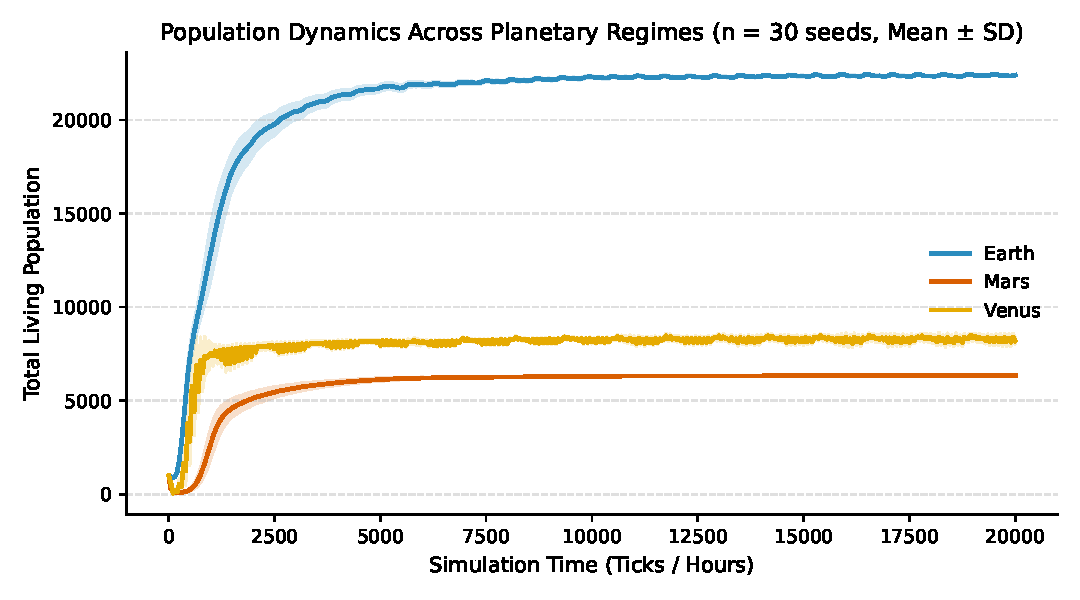
\includegraphics[width=\columnwidth]{data/figures/fig1_population_dynamics.pdf}
    \caption{Mean living population over 20,000 ticks ($n = 30$ seeds, shaded $\pm 1\text{ SD}$). Mars and Venus experience early bottlenecks before stabilizing into distinct equilibria, with Venus displaying 96-hour diurnal oscillations.}
    \label{fig:pop}
\end{figure}

Fig.~\ref{fig:habitat} illustrates complete vertical niche bifurcation: Earth maintains a diverse three-layer biosphere ($33.9\%$ subsurface, $50.2\%$ surface, $15.9\%$ airborne), whereas Mars and Venus both drive surface occupancy to $0.0\%$ (the sole non-significant pairwise comparison in Table~\ref{tab:significance}, $p = 1.0000$), migrating exclusively to opposite vertical extremes ($100\%$ subsurface vs. $100\%$ airborne).

\begin{figure}[t]
    \centering
    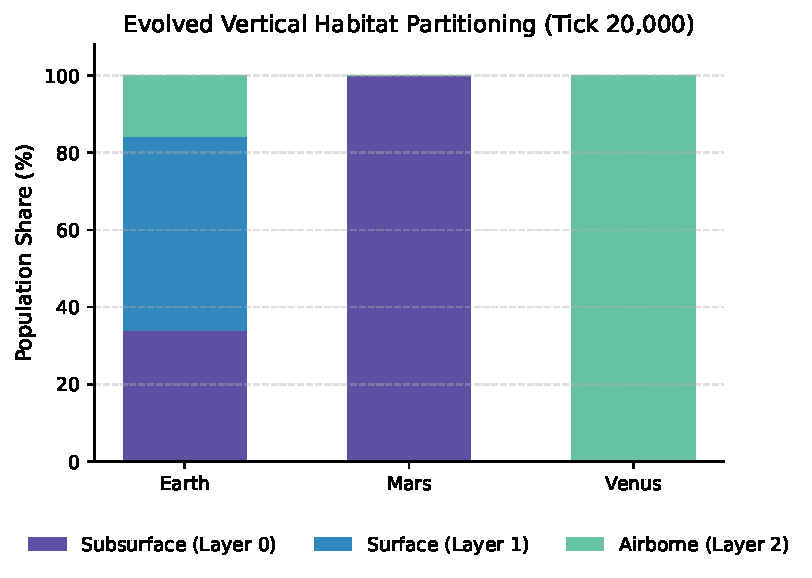
\includegraphics[width=0.92\columnwidth]{data/figures/fig2_habitat_distribution.pdf}
    \caption{Evolved vertical habitat partitioning at tick 20,000. Hostile surface conditions on Mars and Venus eliminate surface life completely, driving opposite vertical specializations.}
    \label{fig:habitat}
\end{figure}

Fig.~\ref{fig:traits} confirms tight convergent evolution across all selected traits ($\text{SD} \le 0.002$ on Mars and Venus). On Mars, populations converged to pure chemosynthesis ($\text{Metab} = 0.008$) and calibrated thermal tolerance ($\text{Therm} = 0.336$) just above the analytical zero-damage threshold of $(|-20 - 20| - 15) / 90 = 0.278$. On Venus, airborne lineages maximized photosynthesis ($\text{Metab} = 0.993$), acid resistance ($\text{Acid} = 0.999$), and dormancy ($\text{Dorm} = 0.953$), while shedding unnecessary thermal tolerance ($\text{Therm} = 0.029$).

\begin{figure}[t]
    \centering
    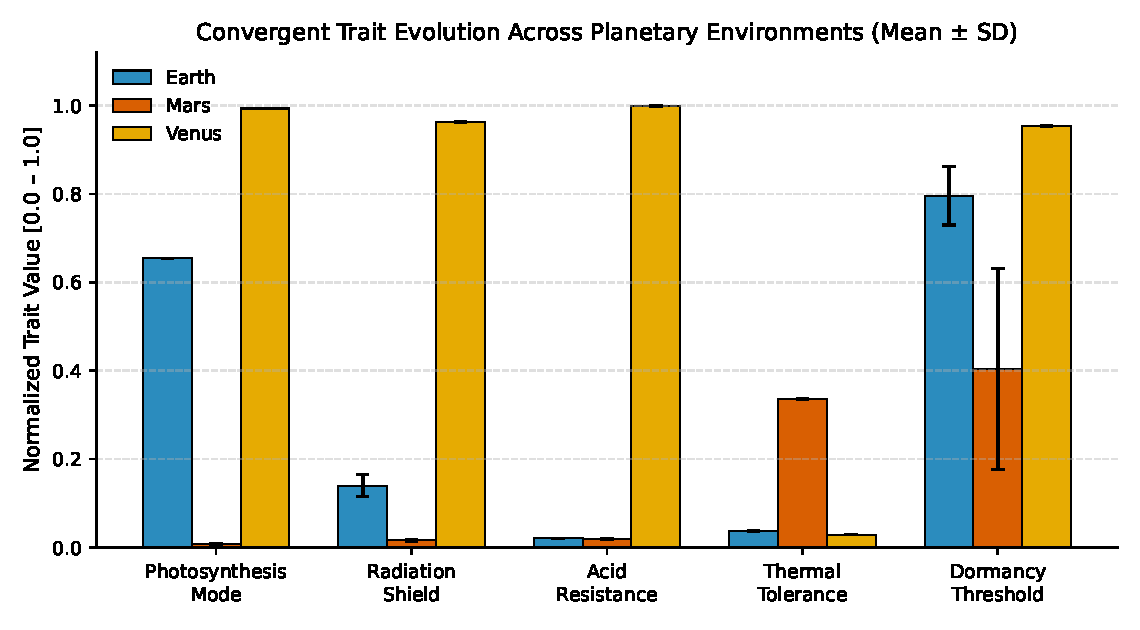
\includegraphics[width=\columnwidth]{data/figures/fig3_trait_convergence.pdf}
    \caption{Convergent trait evolution across planetary environments (mean $\pm 1\text{ SD}$). Tight error bars indicate strong directional selection; the large error bar on Martian dormancy reflects neutral-trait genetic drift.}
    \label{fig:traits}
\end{figure}

\subsection{Sensitivity Analysis and Extinction Tipping Points}
To test model robustness, we ran two parameter sweeps ($n = 10$ seeds/point, $10{,}000$ ticks; Fig.~\ref{fig:sens}):
\begin{enumerate}
    \item \textbf{Mars Subsurface Temperature ($0^\circ\text{C}$ to $-100^\circ\text{C}$):} Evolved thermal tolerance tracked the cooling gradient linearly ($0.117 \rightarrow 0.340 \rightarrow 0.561 \rightarrow 0.786 \rightarrow \approx 0.99$ among survivors at $-80^\circ\text{C}$), matching the analytical slope $\Delta \tau / \Delta T = 20 / 90 = 0.222$ per $-20^\circ\text{C}$. At $-80^\circ\text{C}$, populations hit the biological ceiling ($\tau \approx 1.0$) and entered a stochastic extinction zone ($80\%$ survival), collapsing to $0\%$ at $-100^\circ\text{C}$.
    \item \textbf{Venus Diurnal Cycle ($24\text{ h}$ to $288\text{ h}$):} Extending night length steadily drove radiation shielding upward ($0.820$ at $24\text{ h}$ to $0.945$ at $144\text{ h}$). Between $144\text{ h}$ (72-hour night) and $192\text{ h}$ (96-hour night), the biosphere crossed a sharp extinction cliff, dropping from $100\%$ survival to $0\%$.
\end{enumerate}

\begin{figure*}[t]
    \centering
    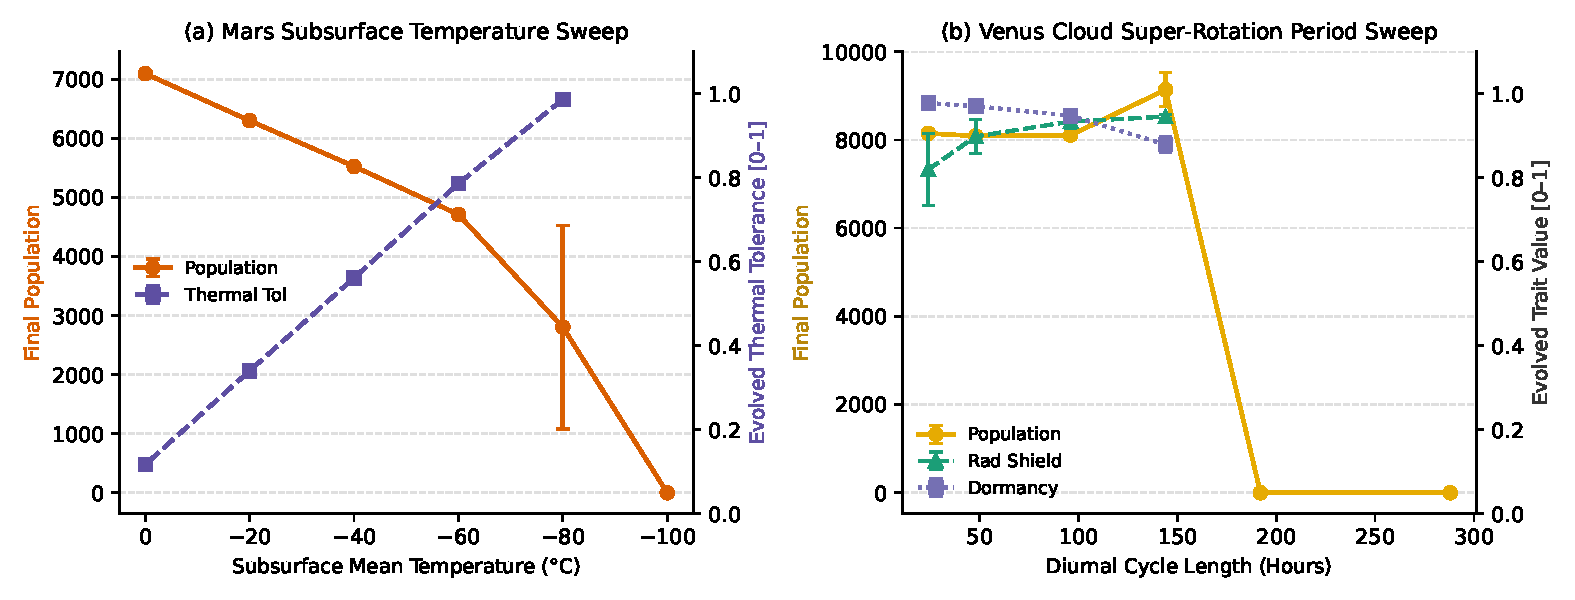
\includegraphics[width=0.92\textwidth]{data/figures/fig4_sensitivity_analysis.pdf}
    \caption{Sensitivity sweeps ($n = 10$ seeds/point, $10{,}000$ ticks). (a) Mars thermal tolerance tracks subsurface cooling linearly until hitting the biological ceiling at $-80^\circ\text{C}$ and collapsing at $-100^\circ\text{C}$. (b) Venusian cloud life requires rising radiation shielding as diurnal periods lengthen, hitting a sharp extinction cliff between 144 and 192 hours.}
    \label{fig:sens}
\end{figure*}

\section{Discussion}
Three emergent findings from our simulation warrant emphasis for computational astrobiology:

\textbf{1) Neutral-Trait Genetic Drift on Mars:} While every actively selected Martian trait exhibited $\text{SD} \le 0.002$, dormancy threshold showed high variance ($\text{SD} = 0.227$; Fig.~\ref{fig:traits}). Because Mars's subsurface provides constant chemosynthetic flux with negligible diurnal amplitude ($\pm 2^\circ\text{C}$), organisms rarely enter energy deficits. Consequently, dormancy becomes selectively neutral and evolves via random genetic drift---an expected population-genetics signature that emerged organically without being hardcoded.

\textbf{2) Nocturnal Radiation Trade-Off on Venus:} Despite modest cloud-deck radiation ($R_2 = 0.15$), Venusian lineages consistently evolved near-maximum radiation shielding ($\text{Rad} = 0.963 \pm 0.002$). Because dormant spores reduce trait upkeep by 75\% overnight while still absorbing unshielded radiation damage, maintaining high radiation armor becomes energetically cheaper than enduring 48 hours of nocturnal damage. The diurnal sweep (Fig.~\ref{fig:sens}b) directly confirms this mechanism: shorter nights relax selection for radiation shielding, whereas nights exceeding 72 hours exhaust spore energy reserves entirely.

\textbf{3) Limitations and Future Work:} Our model abstracts organisms into non-spatial, asexual energy budgets without trophic predation or explicit atmospheric chemistry feedbacks. Future extensions will incorporate 2D spatial dispersal, predator--prey coevolution, and additional ocean-world parameterizations (e.g., Europa and Titan).

\section{Conclusion}
We demonstrated that a deterministic, vectorized agent-based simulator parameterized with real planetary telemetry reliably reproduces astrobiologically consistent niche bifurcation and trait convergence from unbiased initial conditions. Across 90 independent runs and 120 sensitivity trials, simple energy-conservation trade-offs were sufficient to generate Earth-like multi-niche ecosystems, Martian subsurface chemoautotrophs with neutral-trait drift, and acid-resistant Venusian cloud microbes constrained by atmospheric super-rotation. All source code, unit tests, and analysis scripts are openly available for reproduction.

\begin{thebibliography}{9}

\bibitem{seager2021venus}
S.~Seager, J.~J. Petkowski, P.~Gao, W.~Bains, N.~C. Bryan, S.~Ranjan, and J.~Greaves, ``The Venusian lower atmosphere haze as a depot for desiccated microbial life: A proposed life cycle for persistence of the Venusian aerial biosphere,'' \textit{Astrobiology}, vol. 21, no. 10, pp. 1206--1223, 2021.

\bibitem{hassler2014mars}
D.~M. Hassler \textit{et al.}, ``Mars' surface radiation environment measured with the Mars Science Laboratory's Curiosity rover,'' \textit{Science}, vol. 343, no. 6169, p. 1244797, 2014.

\bibitem{adami1998introduction}
C.~Adami, \textit{Introduction to Artificial Life}. New York, NY, USA: Springer-Verlag, 1998.

\bibitem{nasa_factsheet}
D.~R. Williams, ``Planetary Fact Sheet,'' NASA Goddard Space Flight Center, 2024. [Online]. Available: \url{https://nssdc.gsfc.nasa.gov/planetary/factsheet/}

\end{thebibliography}

\end{document}